\section{Additional Graphs \& Diagnostics}\label{app:add_graphs_diags}

% \subsection{Word Count \& Verbosity Bias}\label{app:verbosity_diagnostics}

% \begin{figure}[h]
%     \centering
%     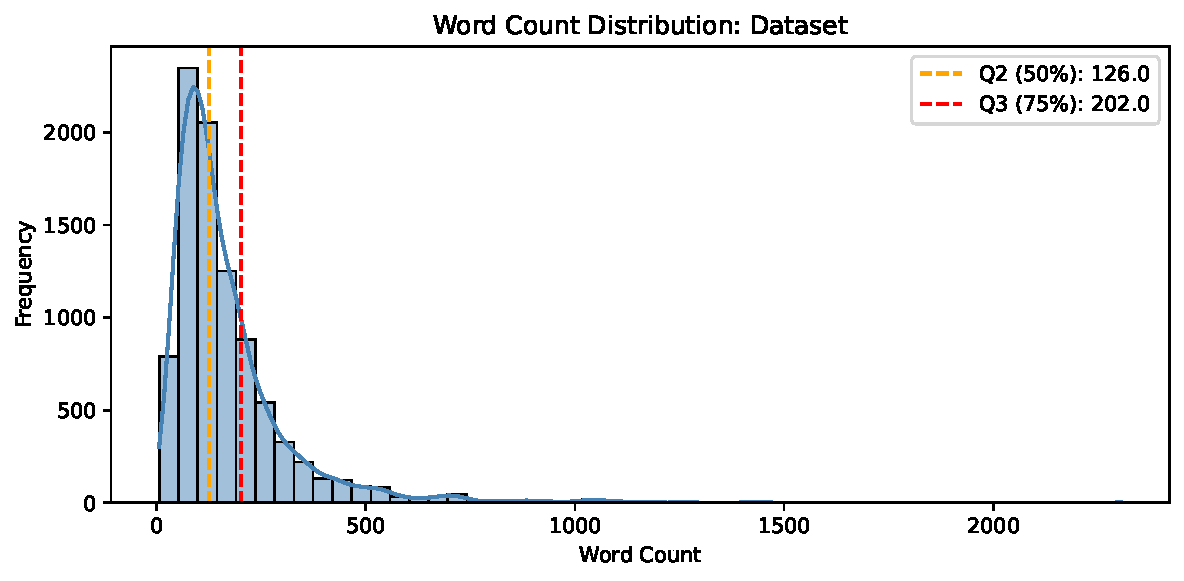
\includegraphics[width=0.8\textwidth]{figures/feedbackqa_word_count.pdf}
%     \caption{Empirical distribution of combined word counts (Question + Answer) for the FeedbackQA dataset. The dashed lines indicate the median ($Q(0.50) = 126$) and the 75th percentile ($Q(0.75) = 202$), which serve as the boundaries for the mature text brackets ($D_{Q3}$ and $D_{Q4}$) used in the verbosity bias assessment.}
%     \label{fig:feedbackqa_word_count}
% \end{figure}

% \begin{figure}[h]
%     \centering
%     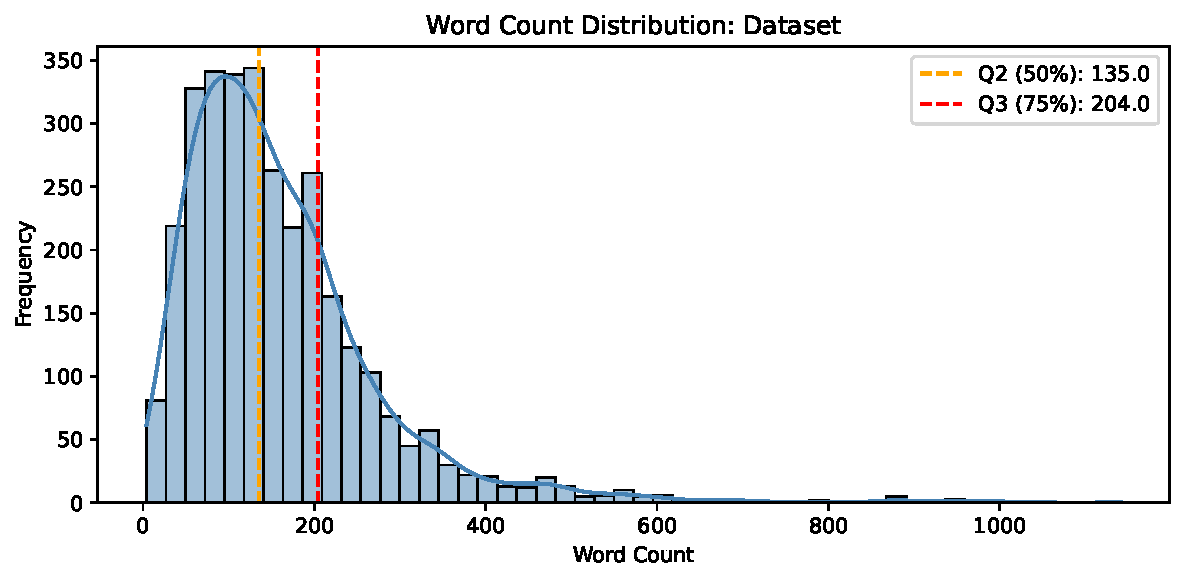
\includegraphics[width=0.8\textwidth]{figures/barter_word_count.pdf}
%     \caption{Empirical distribution of combined word counts (Title + Body + Requirements) for the Barter Deals dataset. The dashed lines indicate the median ($Q(0.50) = 135$) and the 75th percentile ($Q(0.75) = 204$), which serve as the boundaries for the mature text brackets ($D_{Q3}$ and $D_{Q4}$) used in the verbosity bias assessment.}
%     \label{fig:barter_word_count}
% \end{figure}


\subsection{Word Count \& Verbosity Bias}\label{app:verbosity_diagnostics}

\begin{figure}[htbp]
    \centering

    \begin{subfigure}{0.82\textwidth}
        \centering
        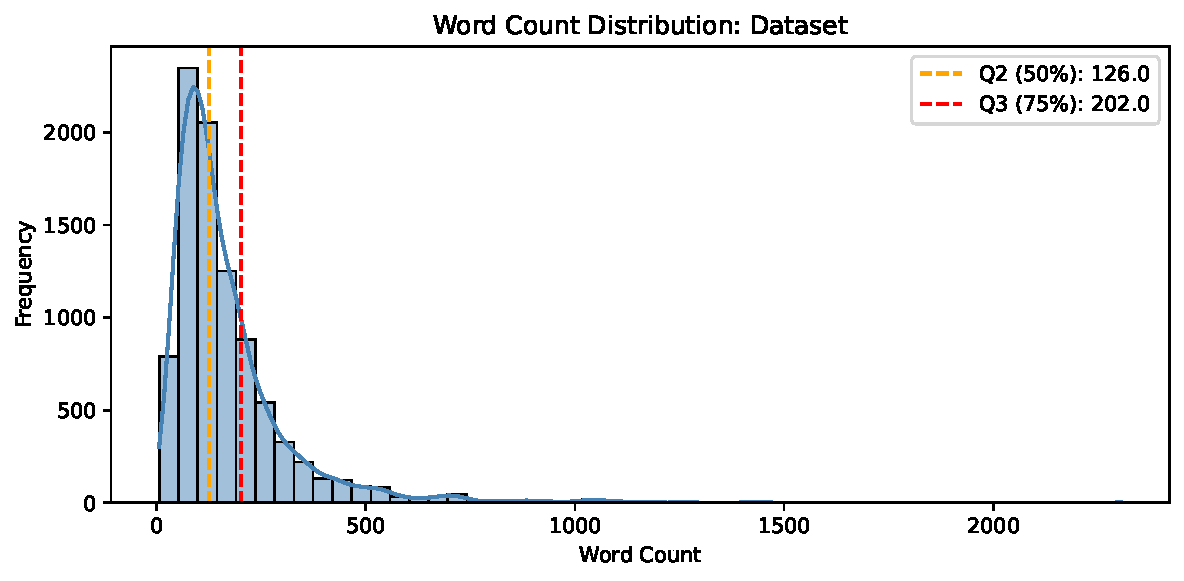
\includegraphics[width=\textwidth]{figures/feedbackqa_word_count.pdf}
        \caption{FeedbackQA: combined word counts (Question + Answer).}
        \label{fig:feedbackqa_word_count}
    \end{subfigure}

    \vspace{0.5em}

    \begin{subfigure}{0.82\textwidth}
        \centering
        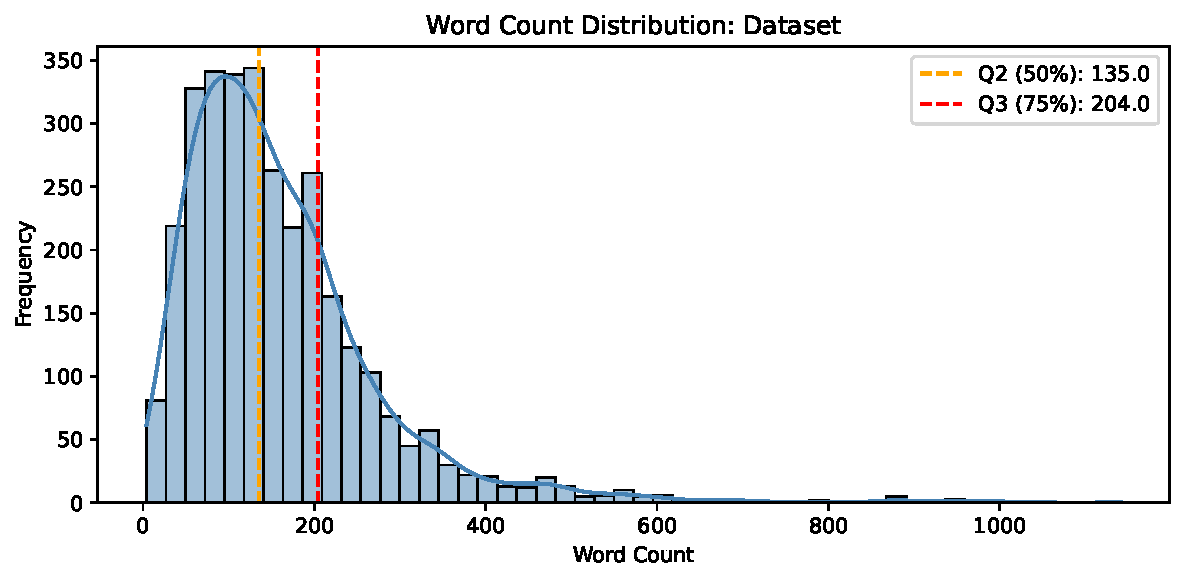
\includegraphics[width=\textwidth]{figures/barter_word_count.pdf}
        \caption{Barter Deals: combined word counts (Title + Body + Requirements).}
        \label{fig:barter_word_count}
    \end{subfigure}

    \caption{Empirical word-count distributions used for the residual verbosity-sensitivity diagnostic. Dashed lines indicate the median and 75th percentile, which define the mature text brackets $D_{Q3}$ and $D_{Q4}$. For FeedbackQA, $Q(0.50)=126$ and $Q(0.75)=202$; for Barter Deals, $Q(0.50)=135$ and $Q(0.75)=204$.}
    \label{fig:word_count_distributions}
\end{figure}



\begin{table}[h]
    \centering
    \caption{Text-length statistics for Barter Deal text sections}
    \label{tab:barter_text_length_stats}
    \begin{tabular}{lrrrr}
    \toprule
    Text Section & Mean Word Count & SD & Median (Q2) & 75th Percentile (Q3) \\
    \midrule
    Body & 81.89 & 72.13 & 64 & 104 \\
    Requirements & 74.92 & 79.55 & 53 & 98 \\
    \bottomrule
    \end{tabular}
\end{table}




\newpage
\subsection{Criterion-Level Rating Distributions}\label{app:rating_distributions}


This subsection reports the full criterion-level EV rating distributions used to support the aggregate rating-regime diagnostics in the main text.

\FloatBarrier

\begin{sidewaysfigure}[p]
    \centering
    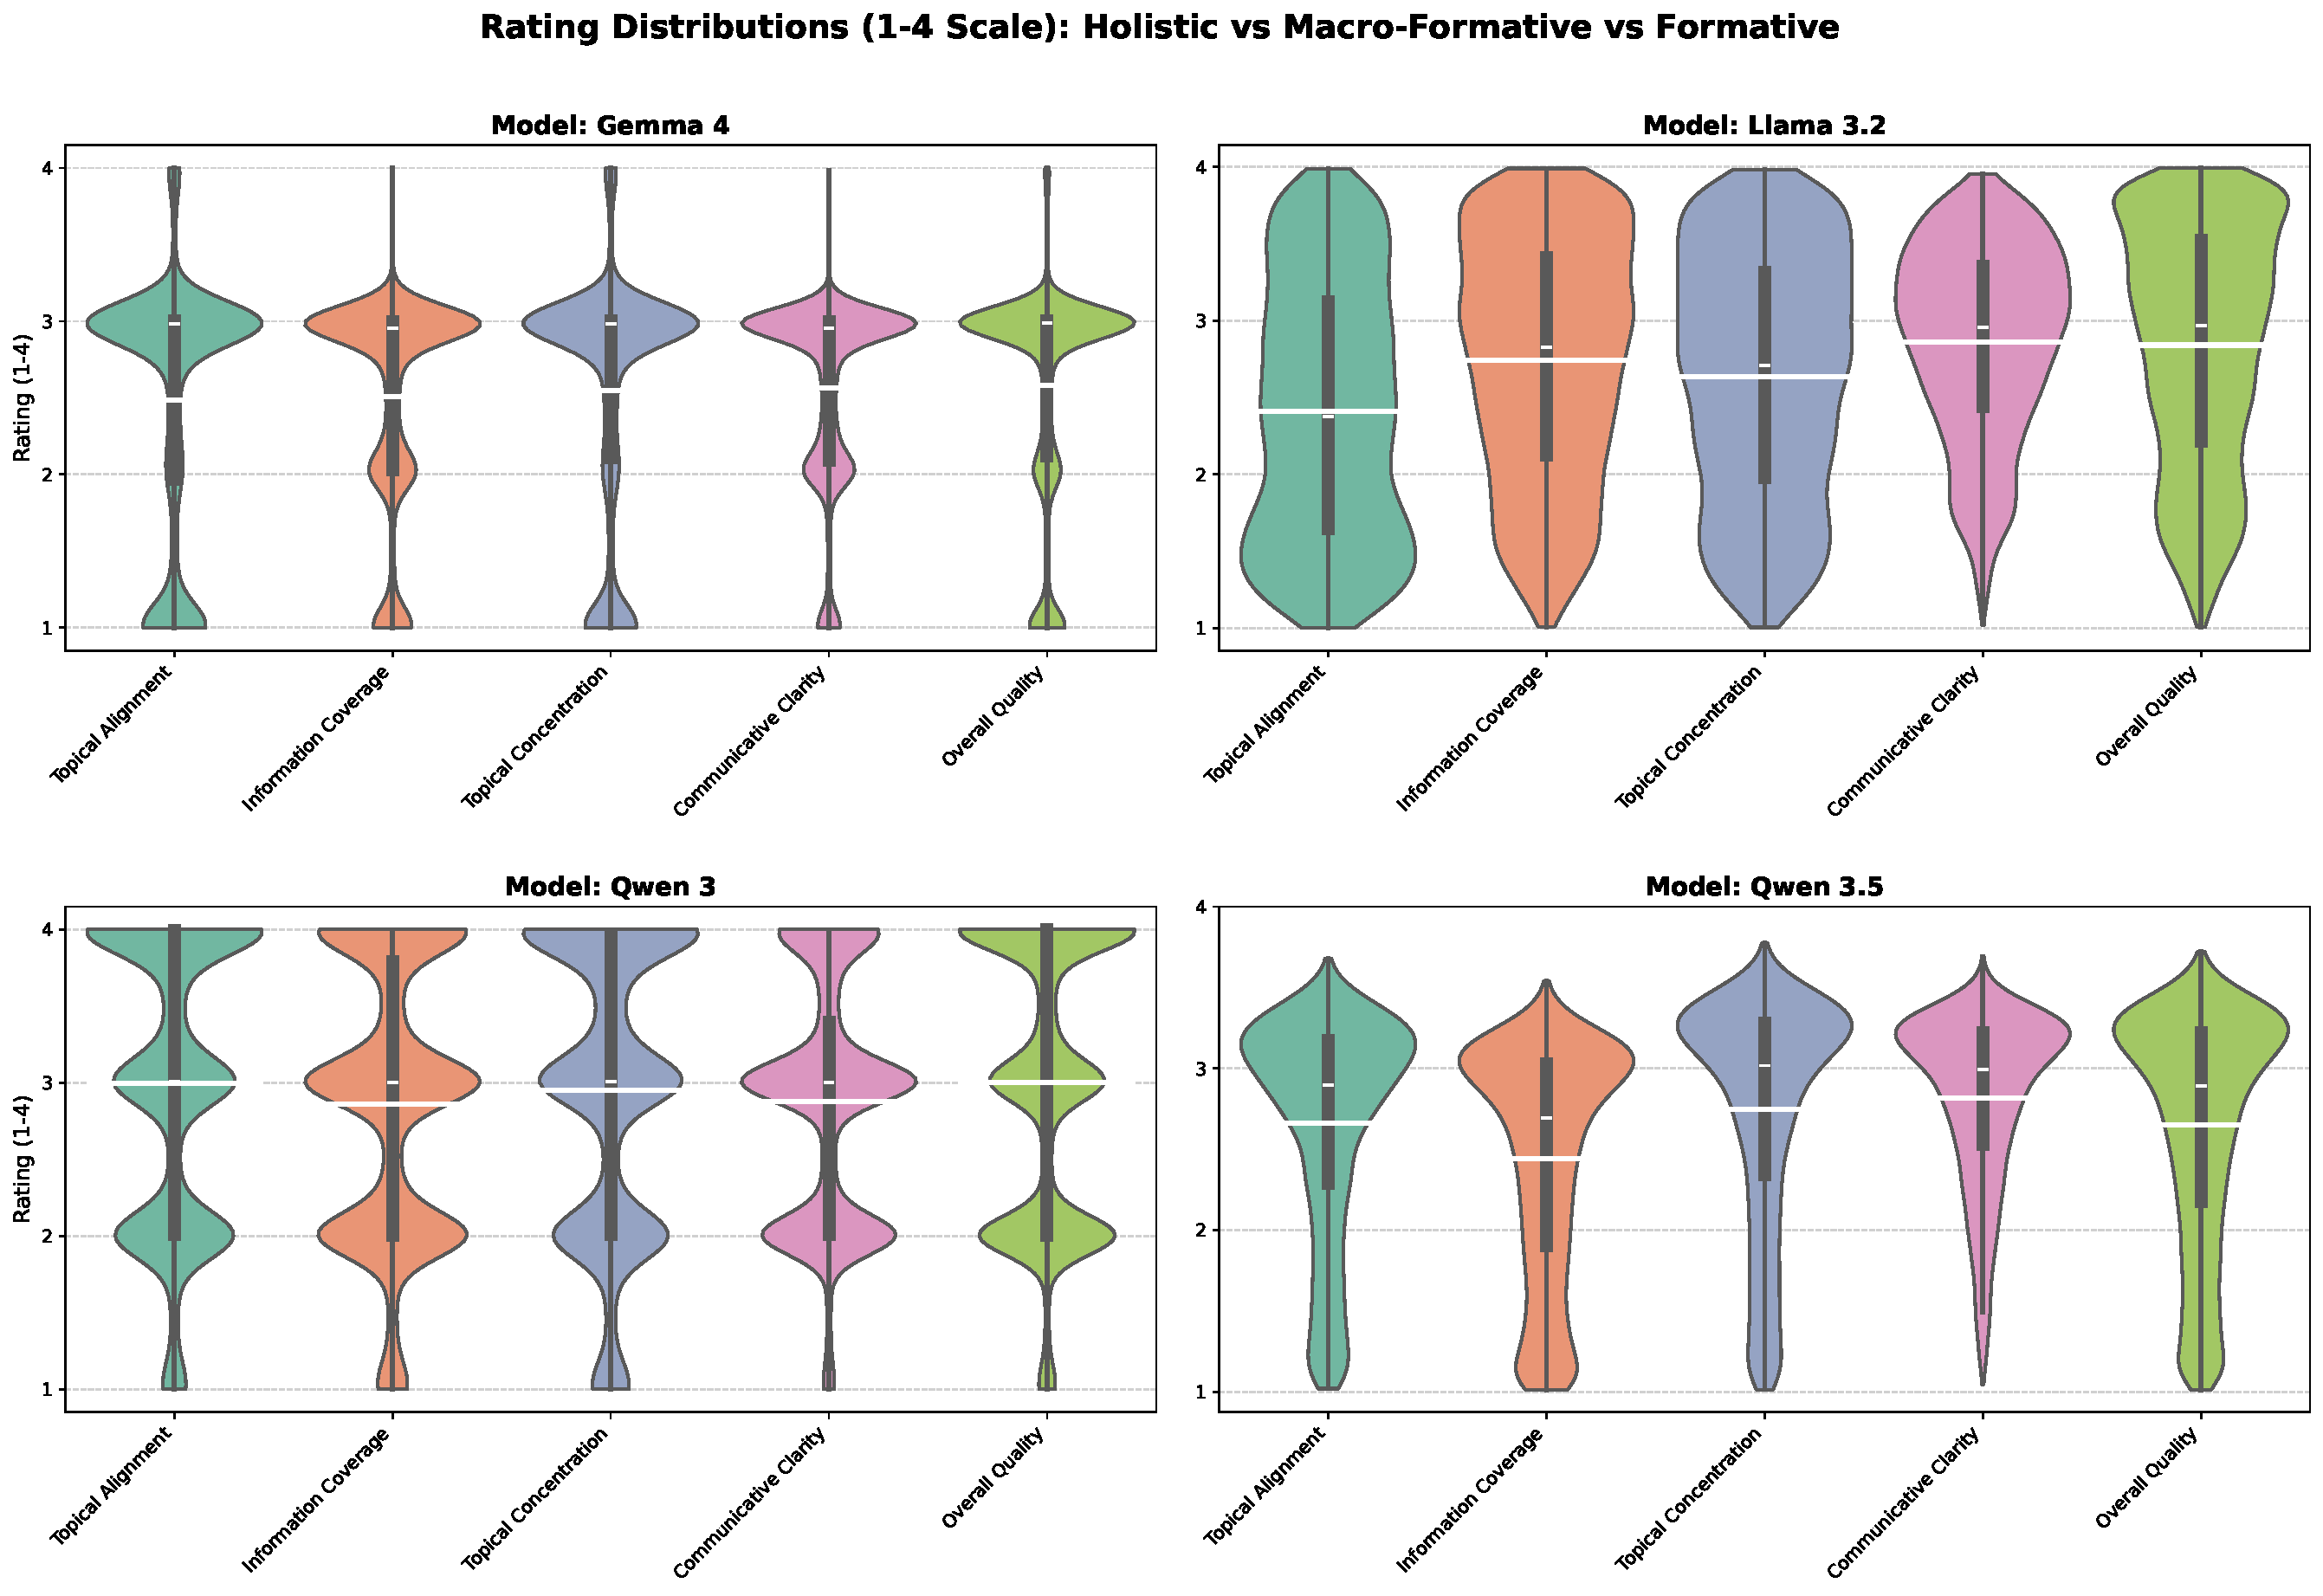
\includegraphics[width=\textwidth]{figures/feedbackqa_rating_distributions.pdf}
    \caption{Criterion-level expected-value rating distributions for Barter Deals.}
    \label{fig:feedbackqa_rating_distributions}
\end{sidewaysfigure}


\begin{sidewaysfigure}[p]
    \centering
    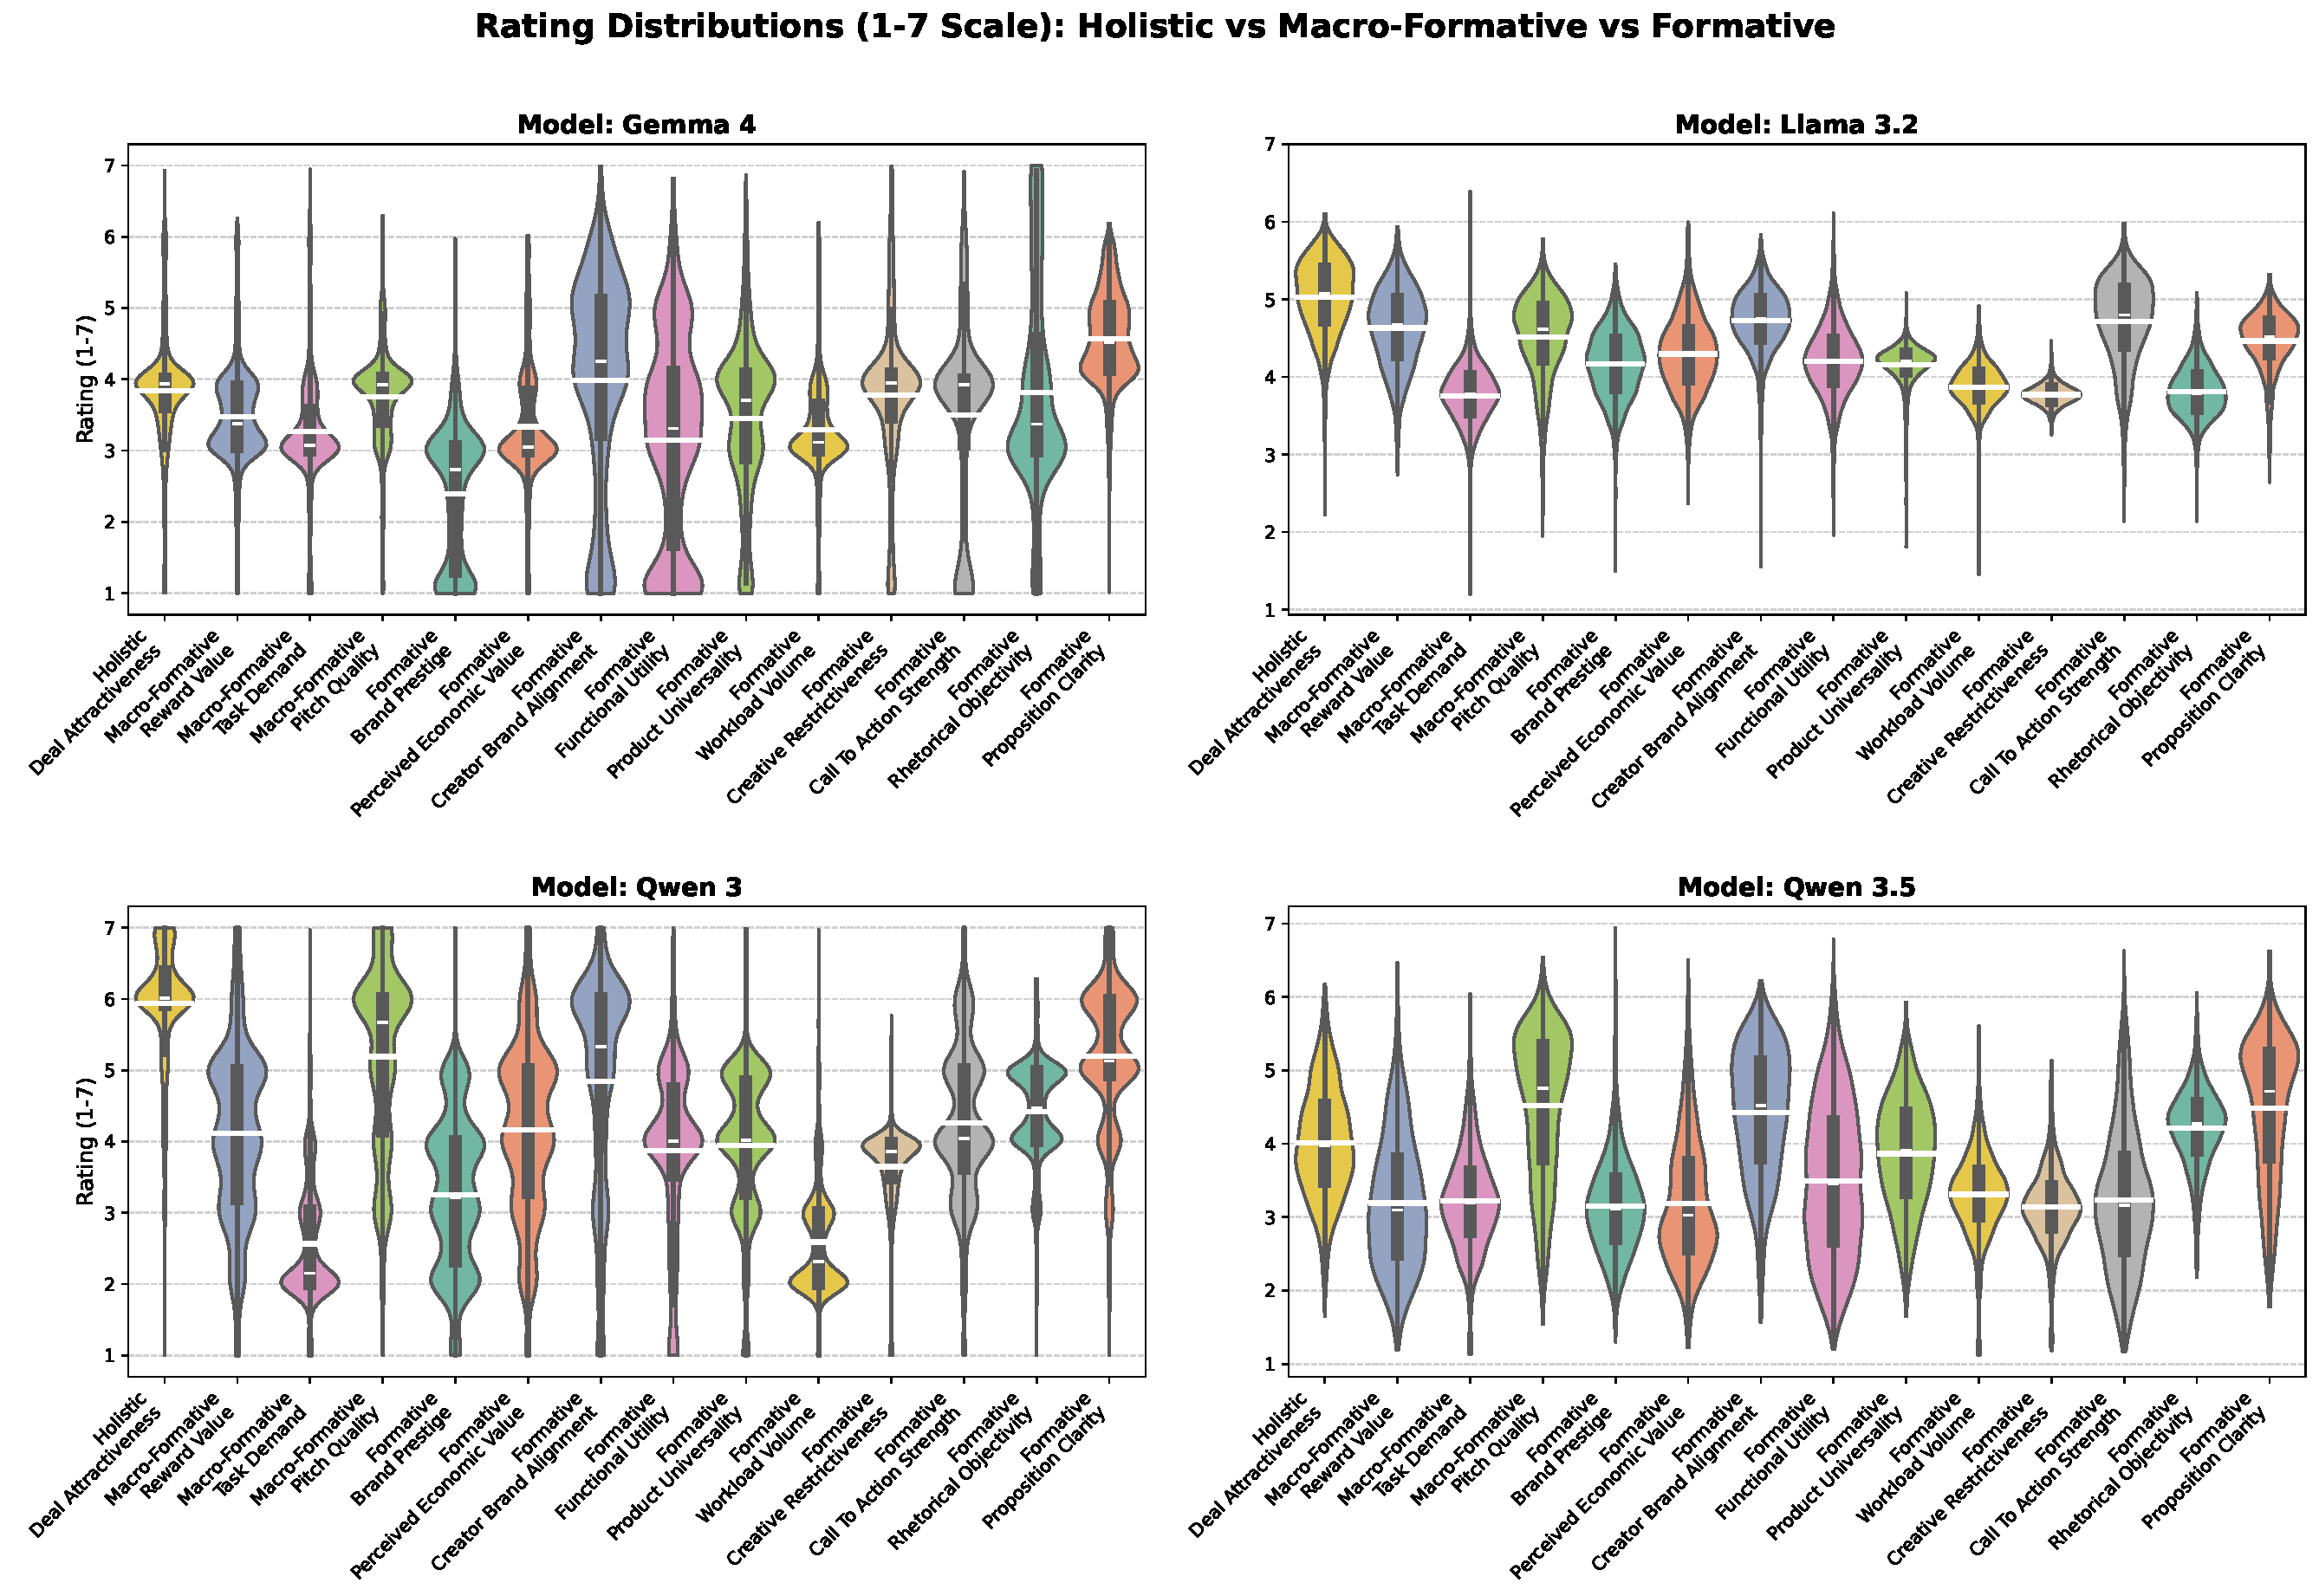
\includegraphics[width=\textwidth]{figures/barter_rating_distributions.pdf}
    \caption{Criterion-level expected-value rating distributions for Barter Deals.}
    \label{fig:barter_rating_distributions}
\end{sidewaysfigure}


\FloatBarrier




\subsection{Additional Multicollinearity Diagnostics}\label{app:vif_diagnostics}

\begin{table}
    \caption{VIF Diagnostics for Barter Deals Formative Specifications}
    \label{tab:VIF_barter}
    \begin{tabular}{lccrrl}
    \toprule
    Group & Max VIF & Mean VIF & N VIF > 5 & N VIF > 10 & Multicollinearity \\
    \midrule
    Gemma 4 Formative & 1.79 & 1.36 & 0 & 0 & Limited \\
    Gemma 4 Macro-Formative & 1.70 & 1.49 & 0 & 0 & Limited \\
    Llama 3.2 Formative & 3.70 & 2.54 & 0 & 0 & Limited \\
    Llama 3.2 Macro-Formative & 4.20 & 2.99 & 0 & 0 & Limited \\
    Qwen 3 Formative & 1.97 & 1.49 & 0 & 0 & Limited \\
    Qwen 3 Macro-Formative & 1.34 & 1.25 & 0 & 0 & Limited \\
    Qwen 3.5 Formative & 2.07 & 1.58 & 0 & 0 & Limited \\
    Qwen 3.5 Macro-Formative & 1.34 & 1.26 & 0 & 0 & Limited \\
    \bottomrule
    \end{tabular}

    \begin{flushleft}
    \footnotesize
    \textit{Note.} VIF values are only computed for the LLM-derived evaluations for the Formative and Macro-Formative conditions, and do not include the non-LLM control variables. Values above 5 are interpreted as moderate multicollinearity and values above 10 as substantial multicollinearity.
    \end{flushleft}
\end{table}


\begin{table}
\centering
\caption{VIF Diagnostics for Barter Deals Baseline Control Specification}
\label{tab:VIF_barter_controls}
\begin{tabular}{lccrrl}
\toprule
Specification & Max VIF & Mean VIF & $N_{\mathrm{VIF}>5}$ & $N_{\mathrm{VIF}>10}$ & Multicollinearity \\
\midrule
Baseline Controls & 5.09 & 2.04 & 1 & 0 & Moderate \\
\bottomrule
\end{tabular}

\begin{flushleft}
\footnotesize
\textit{Note.} VIF values are computed for the non-LLM control specification used in the Barter Deals predictive-validity models. The only predictor exceeding 5 is \textit{macro\_category\_Home Cooking \& CPG} with a VIF of $5.09$. No predictor exceeds 10.
\end{flushleft}
\end{table}


\subsection{Full FeedbackQA Cross-Validation Results}
\label{app:feedbackqa_full_cv}

\paragraph{EV-only model results}

Table~\ref{tab:feedbackqa_cv_full} reports the full set of cross-validated convergent-validity metrics for the FeedbackQA analysis. The main text reports the compact comparison using RMSE and Spearman's $\rho$ only; this appendix table additionally reports Pearson's $r$ and Kendall's $\tau$. The full results confirm the same substantive pattern: the formative condition consistently outperforms the holistic baselines across model architectures, while the informed holistic condition provides only marginal gains over the naive holistic condition.

\begin{table}[htbp]
    \centering
    \caption{Full Cross-Validated Convergent Validity Performance on FeedbackQA}
    \label{tab:feedbackqa_cv_full}
    \begin{tabular}{llcccc}
    \toprule
    Model & Condition & RMSE $\downarrow$ & Pearson's $r$ $\uparrow$ & Spearman's $\rho$ $\uparrow$ & Kendall's $\tau$ $\uparrow$ \\
    \midrule
    Gemma 4 & Holistic Naive & 1.119 & 0.440 & 0.436 & 0.336 \\
    Gemma 4 & Holistic Informed & 1.111 & 0.454 & 0.450 & 0.347 \\
    Gemma 4 & Formative & 1.094 & 0.479 & 0.480 & 0.370 \\
    Llama 3.2 & Holistic Naive & 1.144 & 0.396 & 0.395 & 0.302 \\
    Llama 3.2 & Holistic Informed & 1.144 & 0.397 & 0.396 & 0.302 \\
    Llama 3.2 & Formative & 1.128 & 0.424 & 0.423 & 0.323 \\
    Qwen 3 & Holistic Naive & 1.044 & 0.546 & 0.544 & 0.421 \\
    Qwen 3 & Holistic Informed & 1.039 & 0.553 & 0.550 & 0.426 \\
    Qwen 3 & Formative & 1.018 & 0.577 & 0.578 & 0.449 \\
    Qwen 3.5 & Holistic Naive & 1.033 & 0.559 & 0.559 & 0.435 \\
    Qwen 3.5 & Holistic Informed & 1.034 & 0.558 & 0.558 & 0.434 \\
    Qwen 3.5 & Formative & 1.019 & 0.576 & 0.576 & 0.449 \\
    \addlinespace[0.4em]
    Human-Human & Baseline & 1.196 & 0.542 & 0.541 & 0.467 \\
    \bottomrule
    \end{tabular}

    \begin{flushleft}
    \footnotesize
    \textit{Note.} Values report out-of-fold cross-validated performance for EV-only specifications. RMSE measures prediction error; Pearson's $r$, Spearman's $\rho$, and Kendall's $\tau$ measure alignment with human quality judgments. Lower RMSE and higher correlation coefficients indicate better convergent validity. The human-human baseline compares the two available human annotations and is included as a reference point for annotation consistency, not as a fitted model.
    \end{flushleft}
\end{table}


% \paragraph{Entropy-augmented model results}

% Table~\ref{tab:feedbackqa_entropy_delta} reports the change in cross-validated performance after adding entropy predictors to the EV-only specifications. The changes are uniformly small, confirming that entropy does not materially improve convergent-validity performance beyond the expected-value ratings.

% \begin{table}[h]
% \caption{Change in FeedbackQA Cross-Validation Performance After Entropy Augmentation}
% \label{tab:feedbackqa_entropy_delta}
% \begin{tabular}{llccc}
% \toprule
% Model & Condition & $\Delta$ RMSE & $\Delta r$ & $\Delta \rho$ \\
% \midrule
% Gemma 4 & Holistic Naive & -0.006 & +0.010 & +0.011 \\
% Gemma 4 & Holistic Informed & -0.006 & +0.009 & +0.010 \\
% Gemma 4 & Formative & -0.006 & +0.009 & +0.007 \\
% Llama 3.2 & Holistic Naive & -0.001 & +0.001 & 0.000 \\
% Llama 3.2 & Holistic Informed & 0.000 & 0.000 & 0.000 \\
% Llama 3.2 & Formative & -0.004 & +0.007 & +0.005 \\
% Qwen 3 & Holistic Naive & 0.000 & 0.000 & 0.000 \\
% Qwen 3 & Holistic Informed & 0.000 & 0.000 & 0.000 \\
% Qwen 3 & Formative & 0.000 & 0.000 & 0.000 \\
% Qwen 3.5 & Holistic Naive & -0.003 & +0.003 & 0.000 \\
% Qwen 3.5 & Holistic Informed & -0.003 & +0.004 & +0.001 \\
% Qwen 3.5 & Formative & -0.004 & +0.005 & +0.002 \\
% \bottomrule
% \end{tabular}

% \begin{flushleft}
% \footnotesize
% \textit{Note.} Values report the change from the EV-only specification to the EV+Entropy specification. Negative values indicate improvement for RMSE, while positive values indicate improvement for Pearson's $r$, Spearman's $\rho$, and Kendall's $\tau$. Values close to zero indicate that entropy augmentation does not materially change cross-validated convergent-validity performance.
% \end{flushleft}
% \end{table}


\subsection{Full Barter Deals  Results}
\label{app:barter_full_results}


\paragraph{EV-only model results}

% \paragraph{Entropy-augmented model results}


% \begin{table}[ht]
%     \centering
%     \caption{Incremental Cross-Validated Effect of Entropy Augmentation}
%     \label{tab:barter_entropy_appendix}
%     \begin{tabular}{llrrrr}
%     \toprule
%     Model Family & Condition & $\Delta$RMSE & $\Delta$MAE & $\Delta$Poisson Dev. & $\Delta\rho$ \\
%     \midrule
%     Gemma 4 & Holistic Naive & -0.005 & -0.003 & -0.013 & 0.001 \\
%     Gemma 4 & Macro-Formative & -0.001 & 0.016 & -0.038 & 0.002 \\
%     Gemma 4 & Formative & 0.024 & 0.014 & 0.025 & -0.001 \\
%     Llama 3.2 & Holistic Naive & 0.011 & 0.018 & 0.012 & 0.004 \\
%     Llama 3.2 & Macro-Formative & 0.092 & 0.045 & 0.148 & 0.007 \\
%     Llama 3.2 & Formative & -0.048 & 0.003 & -0.119 & 0.001 \\
%     Qwen 3 & Holistic Naive & 0.020 & 0.012 & 0.007 & 0.000 \\
%     Qwen 3 & Macro-Formative & -0.008 & -0.023 & -0.033 & -0.001 \\
%     Qwen 3 & Formative & 0.020 & 0.021 & 0.063 & 0.002 \\
%     Qwen 3.5 & Holistic Naive & 0.014 & 0.014 & 0.015 & 0.000 \\
%     Qwen 3.5 & Macro-Formative & 0.034 & 0.055 & 0.041 & 0.003 \\
%     Qwen 3.5 & Formative & 0.171 & 0.117 & 0.210 & 0.006 \\
%     \bottomrule
%     \end{tabular}

%     \begin{flushleft}
%     \footnotesize
%     \textit{Note.} Values report the incremental effect of adding normalized entropy to the EV-only specification. $\Delta$RMSE, $\Delta$MAE, and $\Delta$Poisson Dev. are computed as the EV-only value minus the EV+Entropy value; $\Delta\rho$ is computed as the EV+Entropy value minus the EV-only value. Positive values therefore indicate improved cross-validated performance. The entropy effect is treated as exploratory: the largest and most consistent gains occur for the Qwen 3.5 Formative specification, but improvements are not uniform across model families or experimental conditions.
%     \end{flushleft}
% \end{table}
